%% BEACHTE:  C-z C-n  lädt AUC-TeX-Einstellungen!
%=========================================================================
\newif\ifKlein\newif\ifxptAv     % nicht ändern!
%=========================================================================
% DocumentClass-Varianten: Standard-A4, Standard-A5, Verkleinern auf A5:
%-------------------------------------------------------------------------
 \documentclass[11pt,a4paper]{article}
% \documentclass[10pt,a5paper]{article} \Kleintrue\xptAvtrue
% \documentclass[12pt,a4paper,twoside]{article} \Kleintrue\mag 707
%=========================================================================
\ifKlein \AtBeginDvi{\special{papersize=148.5mm,210mm}} \fi
%=========================================================================
% \AtBeginDvi{\special{landscape}}  % für Querformat entkommentieren
%=========================================================================
% schule2e laden:
%-------------------------------------------------------------------------
 % \usepackage[1.2cm,ora,palatinoOSF]{schule2e} 
\usepackage[ora,palatinoOSF]{schule2e} 
%=========================================================================
% Emacs source mit PDFView syncen. NICHT für finale Ausgabe!
%-------------------------------------------------------------------------
% Hier ggf. weitere Pakete einbinden:
%-------------------------------------------------------------------------
 
%=========================================================================
\usepackage{hyperref, breakurl}               %% LETZTES PAKET
%=========================================================================
% \overfullrule=5pt            % Balken bei zu langen Zeilen anzeigen
\parindentOff                % Absätze durch Leerzeile trennen
%=========================================================================

\usepackage{epstopdf}


\newcommand*{\pdifforig}[3][]{\frac{\partial^{#1}{#2}}{\partial^{}{#3}{}^{#1}}}

% Use subscript-writing for partial derivatives
\makeatletter 
\def\ifEmpty#1{\def\@temp{#1}\ifx\@temp\@empty} 
\makeatother

\renewcommand{\vek}[1]{{\bm #1}}
\newcommand{\vv}{\vek{v}}
\newcommand{\laplace}{\triangle}
\newcommand{\sech}{\mathrm{sech}\,}
\newcommand{\cosech}{\mathrm{cosech}\,}
\newcommand{\ind}[1]{_{\mathrm{#1}}}

% \Kopfzeile[n]{{\upshape\jobname.tex}}{}{\MZtoday}

%%================== Ende des Vorspanns ==================================

\begin{document}

\Titelzeile{Programmierprojekt: 2D-Lennard-Jones-Fluid}

\begin{center}
WS 2010/11 -- TU Berlin\\
Theoretische Physik VI (Vertiefung): Statistische Physik I\\
Michael Dacko, Lewin Stein und Christoph Tavan\\
14.02.2011
\end{center}

\section{Umsetzung}
Unsere Simulation implementiert den Leap-Frog-Algorithmus um ein zweidimensionales Lennard-Jones-Fluid mittels Molekulardynamik-Simulation zu untersuchen.

Simuliert wird ein System aus $N$ identischen, kugelförmigen Teilchen der Masse $m$ mit Durchmesser $\sigma$, die über ein beim Abstand $r_c$ abgeschnittenes und geshiftetes Lennard-Jones-Potential der Form
\begin{align}
	U\ind{shift}(r) = 
	\begin{cases} 
	U(r) - U(r_c) - (r - r_c) U'(r_c) & \text{für $r < r_c$},\\ 
	0& \text{sonst}
	\end{cases}
\end{align}
mit
\begin{align}
	U(r)=4 \eps \left[ \left( \frac{\sigma}{r}  \right)^{12} - \left( \frac{\sigma}{r}  \right)^6 \right] \label{eqn:uljnotred}
\end{align}
wechselwirken.

In der gesamten Simulation werden ausschließlich folgende reduzierte Einheiten verwendet:
\begin{alignat*}{2}
t^* &= t \sigma^{-1} (\eps/m)^{1/2} &\quad\quad&\text{Zeit}\\
r^* &= r \sigma^{-1} &\quad\quad&\text{Länge}\\
E^* &= E \epsilon^{-1} &&\text{Energie}\\
v^* &= v (m/\eps)^{1/2} &\quad\quad&\text{Geschwindigkeit}\\
P^* &= P \sigma^3 \epsilon^{-1} &&\text{Druck}\\
\rho^* &= \rho \sigma^3 && \text{Teilchendichte}\\
T^* &= k_B T \epsilon^{-1} && \text{Temperatur}
\end{alignat*}
In diesen Einheiten geschrieben wird das Wechselwirkungspotential (\ref{eqn:uljnotred}) zu
\begin{align}
	U^*(r) = 4 \left[ \left( \frac{1}{r^*}  \right)^{12} - \left( \frac{1}{r^*}  \right)^6 \right] \label{eqn:ulj}.
\end{align}

Die Temperatur im System wird im Gleichgewicht durch die kinetische Energie charakterisiert. Nach Gleichverteilungssatz muss im Gleichgewicht 
\begin{align}
	\left\langle m v_{\alpha}^2 \right\rangle = k_B T
\end{align}
gelten, wobei $v_{\alpha}$ die $\alpha$-Komponente des Geschwindigkeitsvektors eines Teilchens ist. In reduziertein Einheiten ausgedrückt bedeutet das
\begin{align}
	\left\langle {v^*_{\alpha}}^2 \right\rangle = T^*.
\end{align}
Die mittlere quadratische Geschwindigkeit ist also ein direktes Maß für die Temperatur des Systems. Man kann nun für jede Zeit $t$ eine instantane Geschwindigkeit 
\begin{align}
	T^*(t) \equiv \sum_{i=1}^{N} \frac{v^*_i(t)}{N_f} \label{eqn:Tt}
\end{align}
definieren, wobei $N_f = 2N - 2$ die Anzahl der Freiheitsgrade des Systems ist. Zwei Freiheitsgrade müssen abgezogen werden, da wir in der Simulation den Schwerpunkt festhalten. Da wir jedoch immer mindestens $N=100$ Teilchen simulieren wollen, haben wir in allen konkreten Berechnungen stets $N_f \approx 2N$ genähert.

Die instantane Temperatur (\ref{eqn:Tt}) kann nun kontrolliert werden indem alle Geschwindigkeiten mit einem Faktor $\sqrt{ T/T(t)}$ skaliert werden. Diese Methode der Temperatur-Kontrolle setzen wir während der Equilibrierungsphase in unserem Algorithmus ein.

im Folgenden wird der $^*$ der reduzierten Einheiten weggelassen, alle Formelzeichen beziehen sich jeweils auf die reduzierten Einheiten.

\subsection{Initialisierung} % (fold)
\label{sub:initialisierung}
Zunächst werden alle $N$ Teilchen in einer kubischen Anordnung auf die Simulationsbox verteilt. Anschließend bekommt jedes Teilchen eine gleichverteilt zufällige Geschwindigkeit zugewiesen. Die daraus resultierende Schwerpunktsgeschwindigkeit wird berechnet und die Geschwindigkeiten aller Teilchen werden entsprechend angepasst, sodass der Schwerpunkt in Ruhe ist. Die Teilchengeschwindigkeiten werden schließlich wie oben erwähnt mit dem Faktor $\sqrt{ T/T(t)}$ skaliert, sodass sich die gewünschte Temperatur einstellt.

Mit dieser Startkonfiguration wird der MD-Algorithmus gestartet.
% subsection initialisierung (end)

\subsection{MD-Algorithmus} % (fold)
\label{sub:md_algorithms}
In jedem Zeitschritt der Länge $\Delta t$ wird zunächst für jedes Teilchen die auf das Teilchen wirkende Kraft berechnet. Die $x$-Komponente der Kraft ergibt sich beispielsweise zu
\begin{align}
	F_x &= - \pdiff{U}{x} \\
		&= - \pdiff{r}{x} \pdiff{U}{r} \\
		&= - \frac{x}{r} \frac{48}{r} \left[ \left( \frac{1}{r}  \right)^{12} - \frac{1}{2} \left( \frac{1}{r}  \right)^6     \right]  .
\end{align}
An den Rändern der Simulationsbox werden periodische Randbedingungen angenommen.

Anschließend können nach dem Leap-Frog-Schema die Geschwindigkeiten und Orte für den nächsten Zeitschritt berechnet werden:
\begin{align}
	v(t+\Delta t/2) &= v(t-\Delta t/2) + \Delta t F(r(t))\\
	r(t+\Delta t) &= r(t) + \Delta t v(t+\Delta t/2).
\end{align}

Es werden zunächst $n\ind{equil}$ dieser MD-Schritte ausgeführt bis das System im Gleichgewicht ist, hierbei werden die Geschwindigkeiten regelmäßig skaliert um die gewünschte Temperatur einzustellen. Anschließend werden $n\ind{product}$ Schritte ausgeführt. Hierbei werden die statistischen Mittelwerte berechnet, die wir eigentlich suchen. Parallel werden Temperatur und Gesamtenergie sowie deren Mittelwerte ausgegeben um sicherzustellen, dass sich das System im Gleichgewicht befindet (die Mittelwerte sollten konstant sein).
% subsection md_algorithms (end)

\subsection{Berechnung physikalischer Größen} % (fold)
\label{sub:berechnung_physikalischer_groessen}

\minisec{Paarkorrelationsfunktion}
Zur Berechnung der Paarkorrelationsfunktion $g(r)$ wird jedes Teilchen als Mittelpunkt konzentrischer Kreisschalen der Dicke $\Delta r$ angesehen. Nun wird für jede Kreisschale die Anzahl $n(r)$ der Teilchen gezählt, die sich im Abstand zwischen $r$ und $r+\Delta r$ befinden. Daraus lässt sich für jede Kreisschale die lokale Teilchendichte
\begin{align}
	\rho(r) = \frac{n(r)}{2 \pi r \Delta r} 
\end{align}
berechnen. Bezieht man diese lokale Teilchendichte nun noch auf die durschnittliche Dichte $\rho$ des Gesamtsystems erhält man die Paarkorrelationsfunktion
\begin{align}
	\rho(r) = \frac{1}{\rho} \frac{n(r)}{2 \pi r \Delta r}.
\end{align}

\minisec{Druck}
Der Druck wurde direkt aus der Paarkorrelationsfunktion wie in \cite{sperandeo} beschrieben berechnet.
% subsection berechnung_physikalischer_größen (end)

\section{Ergebnisse} % (fold)
\label{sec:ergebnisse}
Sofern nicht anders erwähnt wurden folgende Parameter für die Simulationen verwendet:
\begin{align*}
	N &= 100\\
	T &= 1.8\\
	r_c &= 2.5 \;\text{und}\; 2^{1/6}\\
	\Delta t &= 0.01\\
	n\ind{equil} &= 2000\\
	n\ind{product} &= 6000\\
	\Delta r &= 0.05\\
\end{align*}
Wie Abb. \ref{fig:T_Mean} deutlich zeigt fluktuiert der Mittelwert der Temperatur während der Produktionsphase kaum was ein Zeichen für eine ausreichende Equilibrierung ist. In verschiedenen Simulationsläufen schwankte der Mittelwert der Temperatur allerdings um etwa $5 \%$ um den vorgegebenen Wert von $T = 1.8$.
\begin{figure}[tbp]
 \centering
  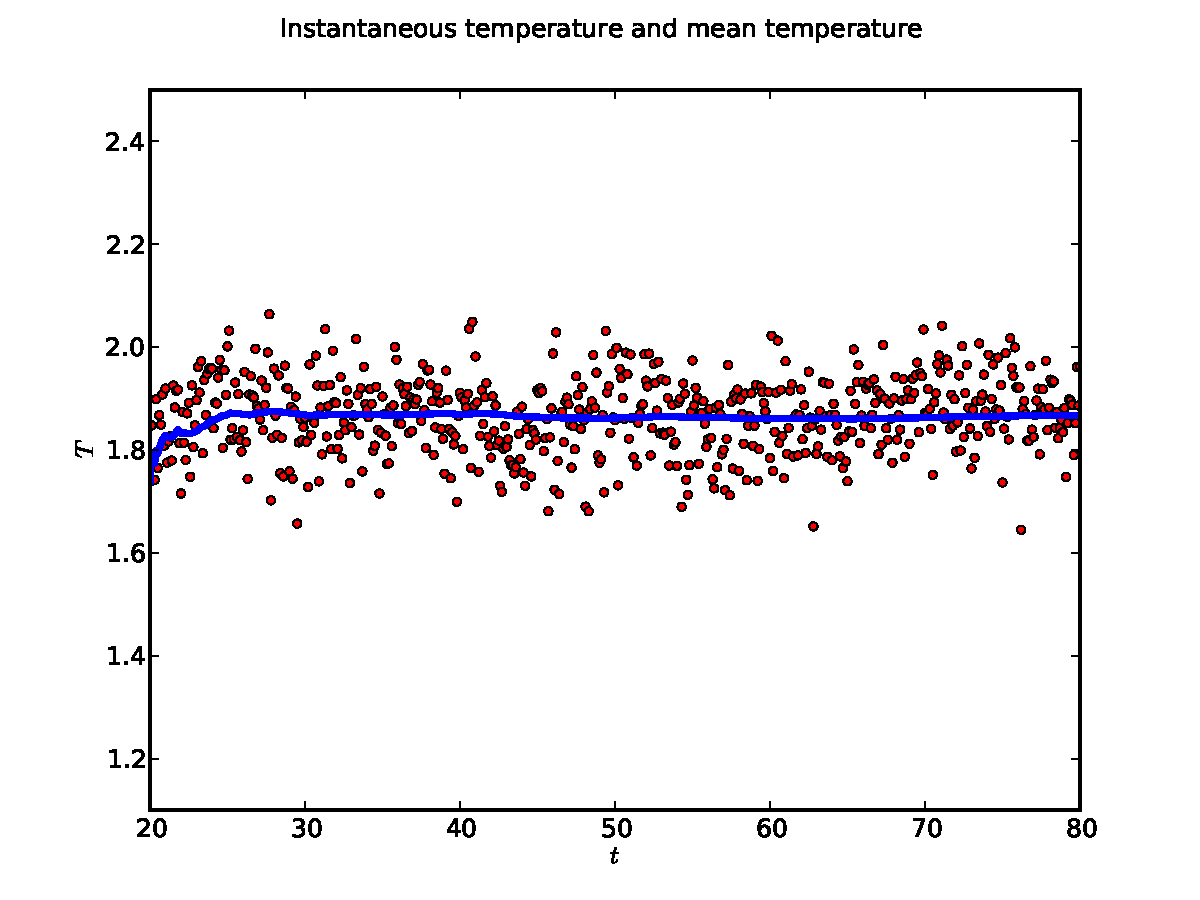
\includegraphics[width=12cm]{../T_mean}
 \caption{Instantane Temperatur und Entwicklung des Mittelwerts der Temperatur während der Produktionsphase bei $\rho = 0.84$.}\label{fig:T_Mean}
\end{figure}

\minisec{Paarkorrelationsfunktion}
Die Paarkorrelationsfunktion ist für drei verschiedene Dichten ist in Abb. \ref{fig:g_r} dargestellt. Sowohl qualitativ als auch quantitativ ergibt sich eine sehr gute Übereinstimmung mit Abb. 3 a) aus \cite{sperandeo}.
\begin{figure}[tbp]
 \centering
  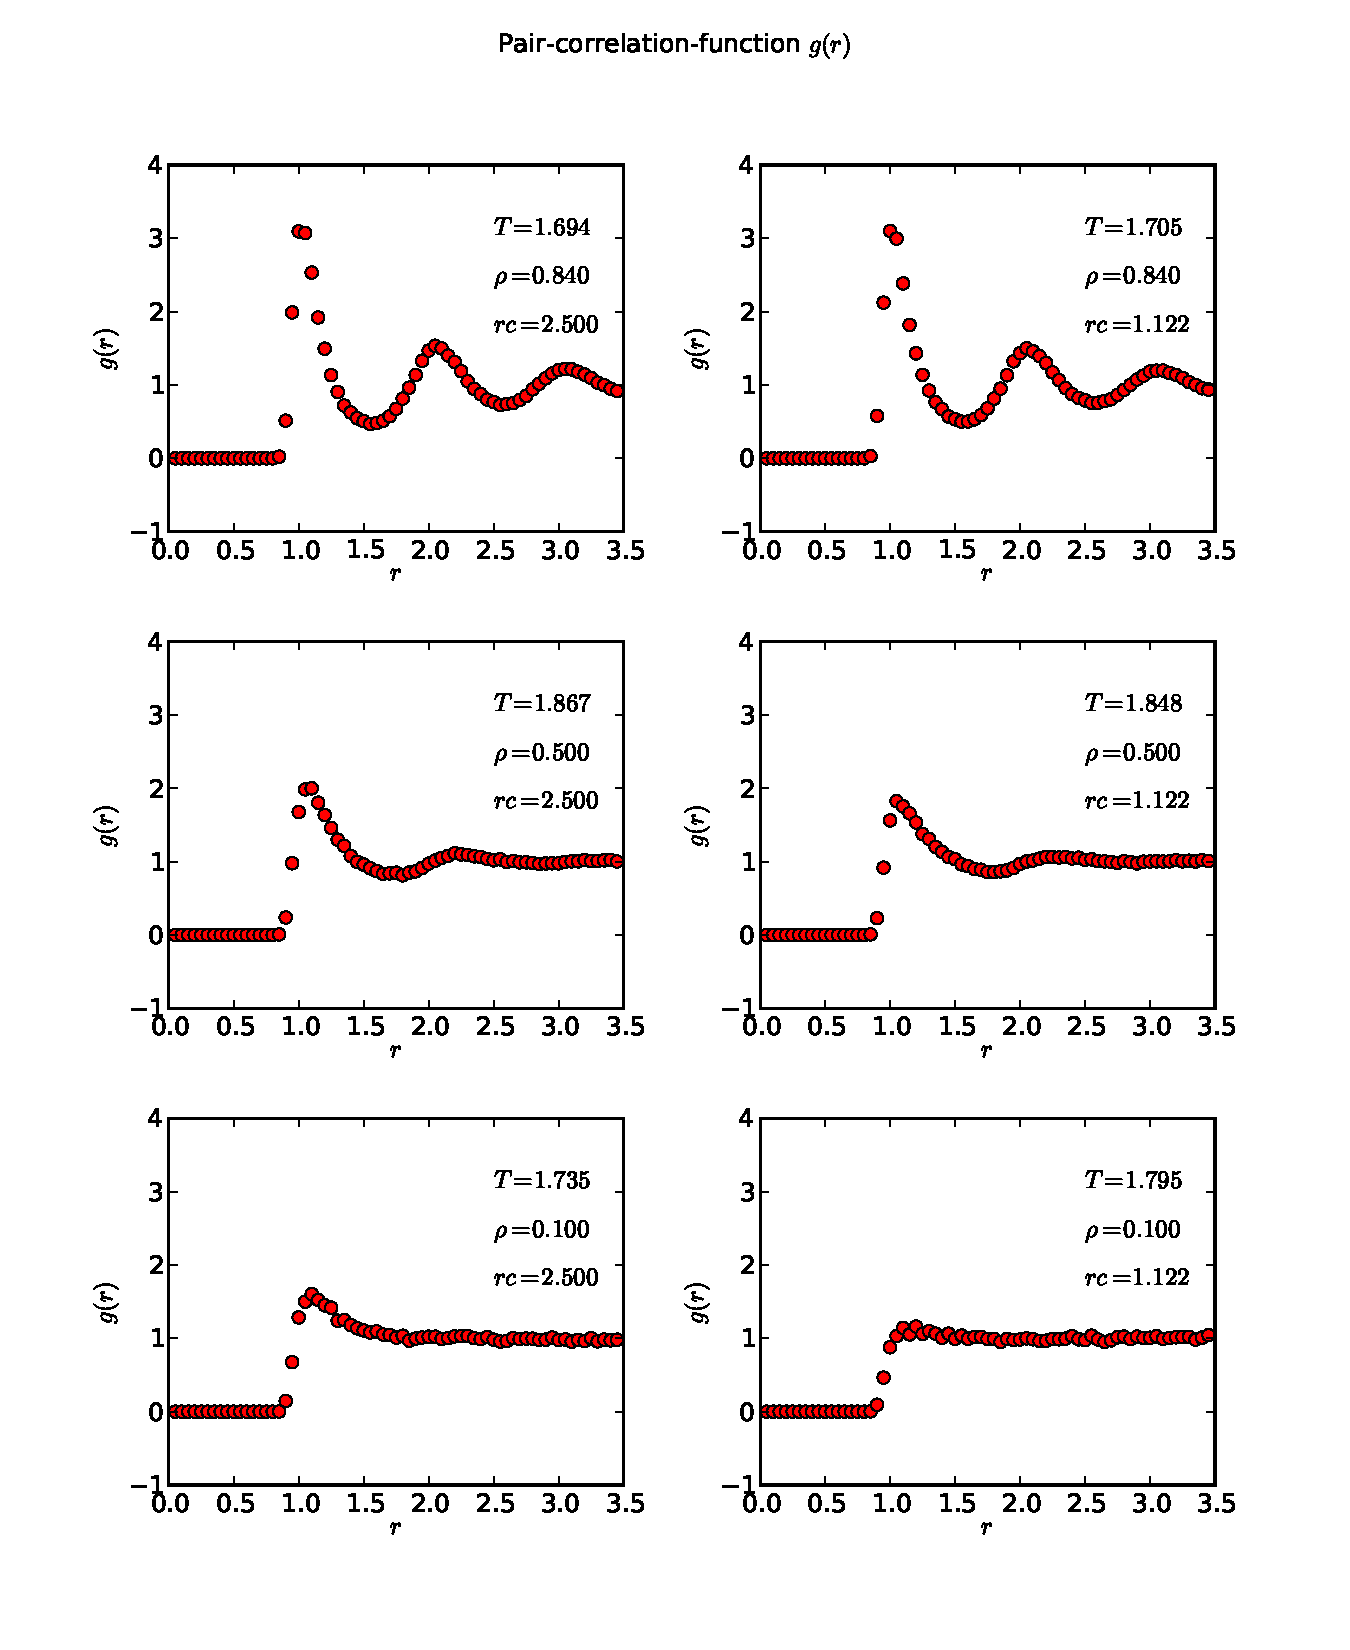
\includegraphics[width=14cm]{../g_r}
 \caption{Paarkorrelationsfunktion $g(r)$ für die Dichten $\rho = 0.84, 0.5$ und $0.1$.}\label{fig:g_r}
\end{figure}

\minisec{Druck}
Wie man Abb. \ref{fig:p_rho} entnehmen kann stimmen auch die Ergebnisse für den Druck qualitativ und quantitativ sehr gut mit Abb. 5 aus \cite{sperandeo} überein.
\begin{figure}[tbp]
 \centering
  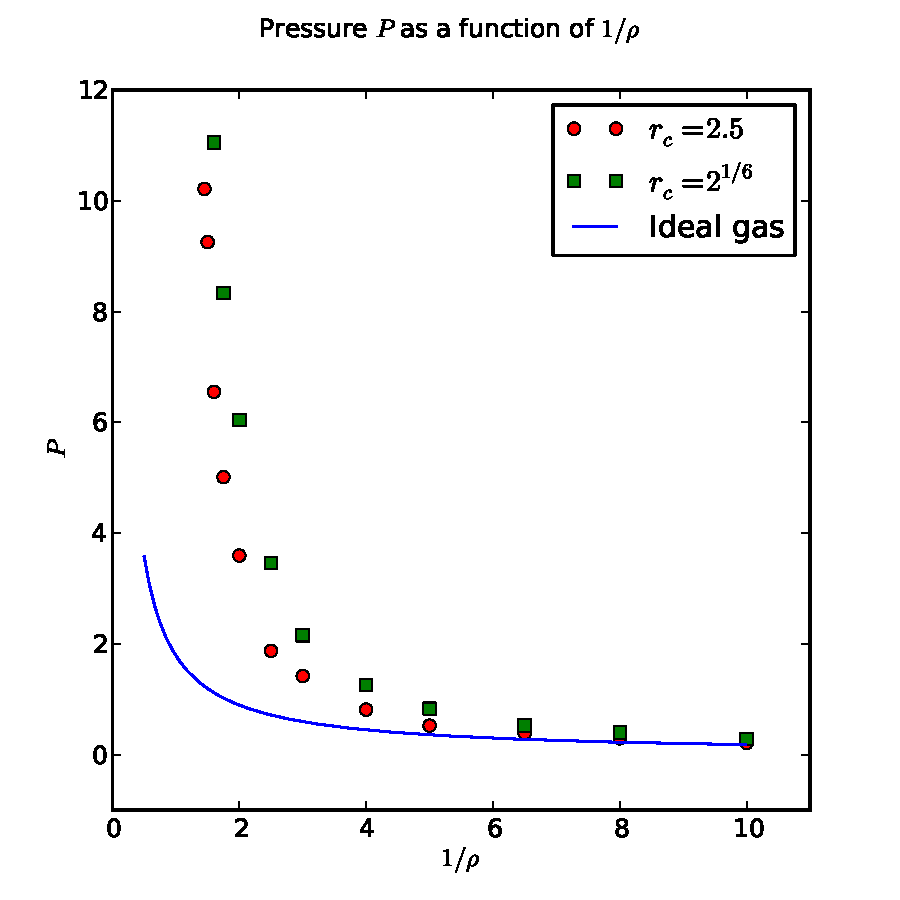
\includegraphics[width=12cm]{../p_rho_T18}
 \caption{Druck $P$ als Funktion der Inversen der Dichte $1/\rho$.}\label{fig:p_rho}
\end{figure}


\minisec{Qualitaet des VdW-Modells}
Auch Abb. 7 aus \cite{sperandeo} konnte zumindest qualitativ reproduziert werden, wie Abb. \ref{fig:vdw} zeigt. Die Druckunterschied sind bei uns quantitativ etwas höher.
\begin{figure}[tbp]
 \centering
  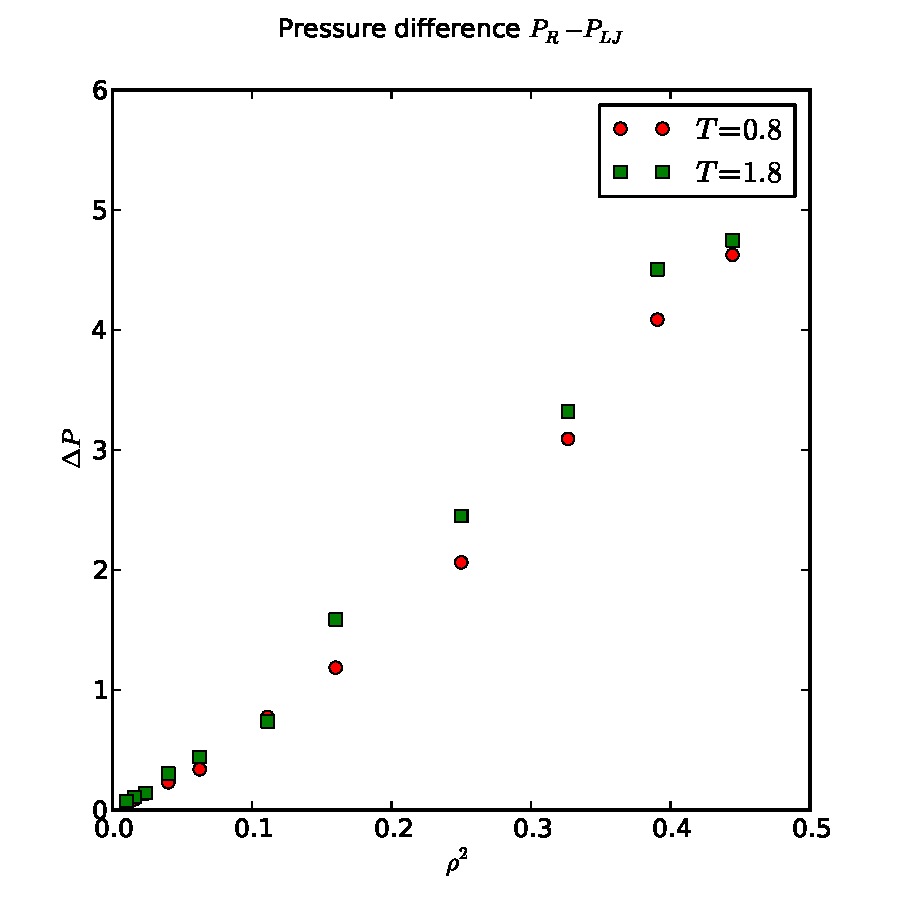
\includegraphics[width=12cm]{../vdw}
 \caption{Druckdifferenz $\Delta P = P_R - P_{LJ}$ zwischen R-Modell ($r_c = 2^{1/6}$) und LJ-Modell ($r_c = 2.5$) als Funktion des Quadrats der Dichte $\rho^2$.}\label{fig:vdw}
\end{figure}
% section ergebnisse (end)


\section{Code} % (fold)
\label{sec:code}
Der Quellcode liegt diesem Text bei und muss im Ordner \texttt{src} via \texttt{make} kompiliert werden. Danach kann man das script \texttt{./run.py} ausführen, das einige Simulationen startet und Plots erstellt.
% section code (end)


%%=================== Ende des Dokuments =================================
% \bibliographystyle{brf-dtk} 
% \bibliography{sfz-Biblio}
\begin{thebibliography}{xx}
	\bibitem{smit} D. Frenkel, B. Smit: \emph{Understanding Molecular Simulations, second edition} Academic Press, Elsevier (2002)
	\bibitem{sperandeo} R. M. Sperandeo-Mineo, G. Tripi: \emph{Microcomputer Simulation of a two-dimensional Lennard-Jones fluid: effects of repulsive and attractive forces.} Eur. J. Phys. \textbf{8}, 117-124 (1984)
\end{thebibliography}
\end{document}